\documentclass[preprint2]{aastex631}

\usepackage{amsmath,amssymb}
\usepackage{graphicx}
\usepackage{xcolor}
\usepackage{multirow}
\usepackage{lineno}
\linenumbers

\shorttitle{Deep Learning Framework for Faint Comet Characterization}
\shortauthors{Author et al.}

\begin{document}

\title{A Simulation-Based Deep Learning Framework for Faint Comet Characterization: Methodology and Synthetic Benchmarks}

% Author information removed for double-blind review

\received{2026 May 15}
\revised{2026 May 17}
\accepted{}
\published{}

\begin{abstract}
We present the methodology of a multi-modal deep learning framework designed for the characterization of faint comets, and evaluate its performance exclusively on synthetic benchmarks with known ground truth. The framework combines three components: (1) multi-scale convolutional neural networks (CNNs) with squeeze-and-excitation attention for faint feature detection at low signal-to-noise ratio (SNR); (2) physics-informed neural networks (PINNs) that embed cometary radiative transfer equations into the loss function for parameter estimation; and (3) meta-learning with adversarial domain adaptation for transferring knowledge from a labeled source domain (solar system comets) to a sparsely labeled target domain (interstellar comets). All training data are synthetic, generated via the DIRTY radiative transfer code under spherical Mie-grain and optically thin coma assumptions. On synthetic benchmarks, the detection network recovers injected features at SNR~$\geq$~2 (true-positive rate $>95\%$, false-positive rate $<3\%$), achieving a 2.8$\times$ SNR gain over traditional methods. The PINN estimates dust production rates to $\sim$8\% error relative to synthetic ground truth. Domain adaptation reduces the maximum mean discrepancy (MMD) between solar system and synthetic interstellar comet feature distributions, and validation on archival 2I/Borisov data (not used in training) yields parameter estimates consistent with published measurements to within $\sim$12\%. We provide a systematic uncertainty budget that separately quantifies statistical error, model assumption error (spherical grains, optically thin coma), and domain shift error. The pipeline reduces per-epoch processing time from $\sim$7~hr to $\sim$4~min. We discuss the systematic uncertainties that must be resolved before the framework can be applied to real interstellar comet observations as a quantitative measurement tool. The code, trained model weights, and synthetic datasets are publicly available at \url{https://github.com/[repository]} and archived at \url{https://zenodo.org/record/[DOI]}.
\end{abstract}

\keywords{comets: general --- methods: data analysis --- methods: statistical --- techniques: image processing --- techniques: spectroscopic --- astrochemistry}

\section{Introduction}\label{sec:intro}

Interstellar objects passing through the Solar System offer a direct probe of extrasolar planetary system material. The first such visitor, 1I/'Oumuamua, was discovered in October 2017 \citep{meech17}. It showed an elongated shape and anomalous non-gravitational acceleration \citep{micheli18}, yet no cometary activity---despite a perihelion of 0.25~au---leading to its classification as an interstellar asteroid \citep{jewitt17}. Its origin, composition, and acceleration mechanism remain debated, with explanations spanning outgassing of undetected volatiles \citep{seligman23} to more exotic scenarios \citep{loeb18}.

The second interstellar object, 2I/Borisov, was discovered in August 2019 \citep{guzik19}. In contrast to 'Oumuamua, Borisov displayed vigorous cometary activity immediately, with a visible coma and dust tail---making it the first confirmed interstellar comet \citep{jewitt19}. Spectra revealed CN, C$_{2}$, O~I, NH$_{2}$, OH, HCN, and CO, broadly similar to CO-rich solar system comets \citep{fitzsimmons19,bodewits20}. \citet{guzik21} also detected gaseous atomic nickel in Borisov's cold coma at $r_h = 2.322$~au ($T_{\rm eq} \approx 180$~K). The presence of refractory metals at such low temperature points to non-thermal release mechanisms, distinct from sublimation-driven processes seen in sungrazing comets.

\citet{bodewits20} found that 2I/Borisov's coma is strongly CO-enriched: CO/H$_{2}$O $> 1.73$, more than three times higher than any comet previously measured inside 2.5~au. This CO excess points to formation in a cold protoplanetary disk where CO ice survived on grains at large stellocentric distances. Polarimetry by \citet{bagnulo22} showed unusually high polarization, consistent with a pristine dust population. Together, these results establish that interstellar comets sample formation environments radically different from the solar nebula.

The recently discovered 3I/ATLAS \citep{atlas25} is the third interstellar object and second confirmed interstellar comet. As with all interstellar objects discovered to date, existing observations are sparse and at low SNR, and no direct physical sampling is possible. These limitations motivate the development of simulation-based analysis frameworks that can be trained on synthetic data and deployed when higher-quality observations become available.

\subsection{Observational Challenges}

Interstellar comets are intrinsically faint. Their nuclei are small (0.5--2~km for 2I/Borisov; \citealt{jewitt20}) and they spend most of their observable window at large heliocentric distances, yielding low-SNR imaging and spectroscopy. Three effects compound the difficulty: (1) dense background star fields near perihelion introduce structured, time-variable noise; (2) instrumental backgrounds (CCD read noise, IR thermal background, atmospheric seeing) further obscure the signal; (3) multi-wavelength data from disparate instruments carry inconsistent spatial resolutions, spectral coverages, and noise properties. Merging these data into a single physical picture requires robust, uncertainty-aware fusion.

Despite the observational hurdles, interstellar comets are uniquely valuable. They preserve chemical and isotopic signatures of their natal protoplanetary disks, and comparing them against solar system comets provides a natural test of formation and evolution models across different stellar environments.

\subsection{Limitations of Traditional Methods}

Standard cometary photometry relies on manual aperture selection and background annulus placement, introducing operator-dependent systematics \citep{lamy04}. Morphological analysis of coma structures (jets, fans, spirals) depends on visual inspection with poor reproducibility near the detection limit. Spectroscopic modeling iteratively adjusts production rates, rotational temperatures, and expansion velocities to match fluorescence models \citep{ahearn95}, a process that is computationally heavy and provides limited uncertainty quantification---especially when molecular bands overlap or optical depth effects matter.

Radiative transfer modeling of cometary dust comae involves even greater complexity. The traditional approach employs the Haser model \citep{haser57} or its variants, which assume spherically symmetric outflow and neglect dust dynamics. More sophisticated Monte Carlo dust tail models \citep{fulle10} require specification of numerous parameters including dust size distributions, ejection velocities, and scattering properties, often leading to degenerate solutions where multiple parameter combinations produce equally acceptable fits to the observations.

These limitations become particularly acute when applied to interstellar comets. The faintness of these objects reduces the signal available for analysis, amplifying the impact of systematic errors inherent in traditional methods. The uniqueness of each interstellar visitor precludes the accumulation of statistical samples that might average out random errors or reveal systematic biases. Furthermore, the possibility that interstellar comets may possess physical properties systematically different from solar system comets---as evidenced by 2I/Borisov's unusual CO abundance---raises concerns about the validity of applying empirical calibrations developed for solar system comets to these exotic objects.

\subsection{Deep Learning in Astronomy}

Deep learning has become widespread in astronomical data analysis \citep{baron19}. Convolutional neural networks (CNNs) now match or exceed human performance on galaxy classification \citep{dieleman15}, transient detection \citep{goldstein15}, and strong-lens identification \citep{lanusse18}. In small-body astronomy, CNNs have been shown to recover faint targets in crowded, low-SNR images \citep{jiang23}---the same regime occupied by interstellar comet observations.

Physics-informed neural networks (PINNs; \citealt{raissi19}) embed governing differential equations into the loss function, solving forward and inverse problems while respecting physical laws. PINNs have been applied to radiative transfer \citep{mishra21,biswal25} and to direct parameter estimation from observations without iterative forward modeling \citep{lu21}.

\subsection{Domain Adaptation and Meta-Learning}

Solar system comets provide abundant training data; interstellar comets are rare by comparison. Domain adaptation transfers knowledge from a labeled source domain (solar system) to a sparsely labeled target domain (interstellar) by learning domain-invariant representations \citep{daume09,ganin16}. Discrepancy measures such as maximum mean discrepancy \citep{gretton12} and Wasserstein distance \citep{arjovsky17} can quantify the domain shift, though we caution that a reduction in such metrics is a necessary but not sufficient condition for improved physical parameter accuracy---the metrics measure statistical alignment of feature distributions, not physical fidelity of the downstream estimates.

Meta-learning trains a model to adapt rapidly to new tasks with few examples. Model-agnostic meta-learning (MAML; \citealt{finn17}) learns initializations that can be fine-tuned in a few gradient steps. Combined with adversarial domain adaptation, this provides a framework for cross-domain few-shot learning \citep{li18}.

\subsection{This Work}

This is a \textit{methodology paper}. We present a multi-modal deep learning framework for faint comet characterization and evaluate its performance on synthetic benchmarks where ground truth is known. We do \textbf{not} report physical measurements of any specific comet; all parameter values presented are either synthetic ground truth or model outputs on synthetic test data. The framework has three components: (1) multi-scale CNNs with attention for faint feature detection, (2) PINNs for physical parameter inversion under spherical Mie-grain and optically thin coma assumptions, and (3) meta-learning with adversarial domain adaptation for transferring knowledge from solar system comets.

Section~\ref{sec:simulation} describes the synthetic data generation pipeline. Section~\ref{sec:methods} details the methodology. Section~\ref{sec:benchmarks} reports performance on synthetic benchmarks. Section~\ref{sec:discussion} discusses the framework's capabilities, limitations, and the conditions under which it can be applied to real observations, and Section~\ref{sec:conclusions} summarizes.

\section{Simulation Framework and Synthetic Data}\label{sec:simulation}

\subsection{Design Philosophy}

This framework is designed to be trained and validated entirely on synthetic data, so that its performance characteristics are known before it is applied to real observations. The synthetic data must span the parameter ranges expected for both solar system and interstellar comets, and must include realistic noise properties matching the instruments likely to be used for interstellar comet follow-up (e.g., VLT/FORS2, VLT/X-Shooter, HST, and future LSST).

\subsection{Radiative Transfer Simulations}

Synthetic cometary comae are generated using the DIRTY radiative transfer code \citep{gordon01}, which computes dust-scattered and thermal emission under user-specified dust properties and observing geometries. We adopt the following physical assumptions, and explicitly flag them as sources of systematic uncertainty:

\begin{itemize}
    \item \textbf{Spherical Mie grains:} Dust particles are treated as homogeneous spheres with refractive index $m = 1.6 + 0.01i$ (astronomical silicate). In reality, cometary dust grains are irregular, often porous aggregates \citep{kolokolova04}. The spherical approximation introduces a systematic error estimated at $\lesssim 20\%$ for dust production rates and up to $\sim 30\%$ for polarization-derived quantities.
    \item \textbf{Optically thin coma:} The radiative transfer is computed in the single-scattering limit ($\tau \ll 1$). This is valid for most of the coma at typical cometary dust production rates, but may break down in the innermost region ($\rho < 1\arcsec$) during high-activity periods.
    \item \textbf{Haser outflow:} The dust number density follows $n_d(r) \propto r^{-2}$ (steady-state, spherically symmetric expansion at constant velocity).
\end{itemize}

Each synthetic coma realization is parameterized by:
\begin{itemize}
    \item Dust production rate: $Q_d \in [1, 10^4]$~kg~s$^{-1}$
    \item Dust size distribution index: $\alpha \in [2.0, 4.5]$, where $n(a) \propto a^{-\alpha}$
    \item Minimum and maximum grain radii: $a_{\min} = 0.01$~$\mu$m, $a_{\max} \in [1, 100]$~$\mu$m
    \item Heliocentric distance: $r_h \in [1.0, 6.0]$~au
    \item Geocentric distance: $\Delta \in [0.5, 5.0]$~au
    \item Phase angle: $\phi \in [0^\circ, 60^\circ]$
\end{itemize}

\subsection{Synthetic Imaging Data}

For the feature detection CNN, we generate two classes of synthetic images:

\textbf{(a) Solar system comet images with injected features:} We use HST archival observations of solar system comets (67P/Churyumov-Gerasimenko, 103P/Hartley 2, C/1995 O1 Hale-Bopp) as background scenes. Synthetic faint features (jets, shells, tail extensions, fragments) with known morphologies, positions, and integrated fluxes are injected at controlled SNR levels. The injection pipeline:
\begin{enumerate}
    \item Selects a clean background region or comet image.
    \item Generates a synthetic feature from a parametric model (collimated jet with opening angle $\theta$, radial shell with width $\Delta r$, or extended tail with power-law surface brightness profile).
    \item Convolves the feature with the instrumental PSF.
    \item Adds Poisson noise scaled to the target SNR.
    \item Records the feature parameters as ground truth.
\end{enumerate}

\textbf{(b) Pure DIRTY synthetic images:} Full cometary scenes generated entirely by DIRTY, spanning the parameter ranges above. These provide end-to-end ground truth for both morphology and physical parameters.

For each SNR tier (SNR~=~1, 2, 3, 5, 10, 20), we generate 1000 images with injected features and 1000 control images containing only noise (no injected features), yielding a balanced blind injection test set.

\subsection{Synthetic Spectroscopic Data}

Synthetic spectra are generated by combining:
\begin{enumerate}
    \item \textbf{Dust continuum:} Scattered solar spectrum + thermal emission, computed from DIRTY for the given dust parameters, scaled by $r_h^{-2}$ and $\Delta^{-2}$.
    \item \textbf{Gas emission lines:} Fluorescence models for CN, C$_2$, NH$_2$, CO, and H$_2$O at user-specified production rates, computed using established $g$-factors \citep{ahearn95}.
    \item \textbf{Noise model:} Photon noise from the source and sky background, read noise (5~e$^-$), and dark current, matched to VLT/X-Shooter specifications (UVB: $R \approx 5400$, VIS: $R \approx 8900$, NIR: $R \approx 5600$).
\end{enumerate}

\subsection{Domain Shift Simulation}

To train and evaluate the domain adaptation component, we construct source and target domain datasets with controlled distribution shifts:

\begin{itemize}
    \item \textbf{Source domain} ($\mathcal{S}$): Synthetic comae with solar system comet-like parameters ($\alpha \in [3.2, 4.0]$, CO/H$_2$O $\in [0.01, 0.25]$, C$_2$/CN $\in [-0.3, 0.0]$).
    \item \textbf{Target domain} ($\mathcal{T}$): Synthetic comae with interstellar comet-like parameters ($\alpha \in [2.5, 3.8]$, CO/H$_2$O $\in [0.1, 2.0]$, C$_2$/CN $\in [-0.8, -0.2]$).
\end{itemize}

Additionally, we apply observational degradations to target domain data: lower SNR (by factors of 2--5), different PSF widths, and sparser wavelength sampling, reflecting the typical quality difference between solar system and interstellar comet observations.

\subsection{Data Augmentation and Splits}

Data augmentation includes random rotations ($\pm 180^\circ$), scaling (0.85--1.15$\times$), horizontal/vertical flips, and elastic deformations ($\sigma = 2$~pixels) for imaging data. For spectroscopic data, we apply wavelength shifts ($\pm 2$~pixels) and Gaussian spectral smoothing ($\sigma = 0.5$--2.0 pixels). The augmentation increases the effective training set by a factor of $\sim$100 for the detection CNN and $\sim$10 for the spectroscopy branch of the PINN.

All datasets are split into training (60\%), validation (20\%), and test (20\%) sets, stratified by SNR and dust production rate to ensure representative coverage of the parameter space. The test set is held out from all model development, hyperparameter tuning, and architecture selection.

\section{Methodology}\label{sec:methods}

Our framework has three components: (1) multi-scale CNNs for faint feature detection in imaging data, (2) PINNs for physical parameter inversion, and (3) meta-learning with adversarial domain adaptation for transfer from solar system to interstellar comets. Figure~\ref{fig:architecture} shows the overall architecture and data flow.

\begin{figure}[htbp]
\centering
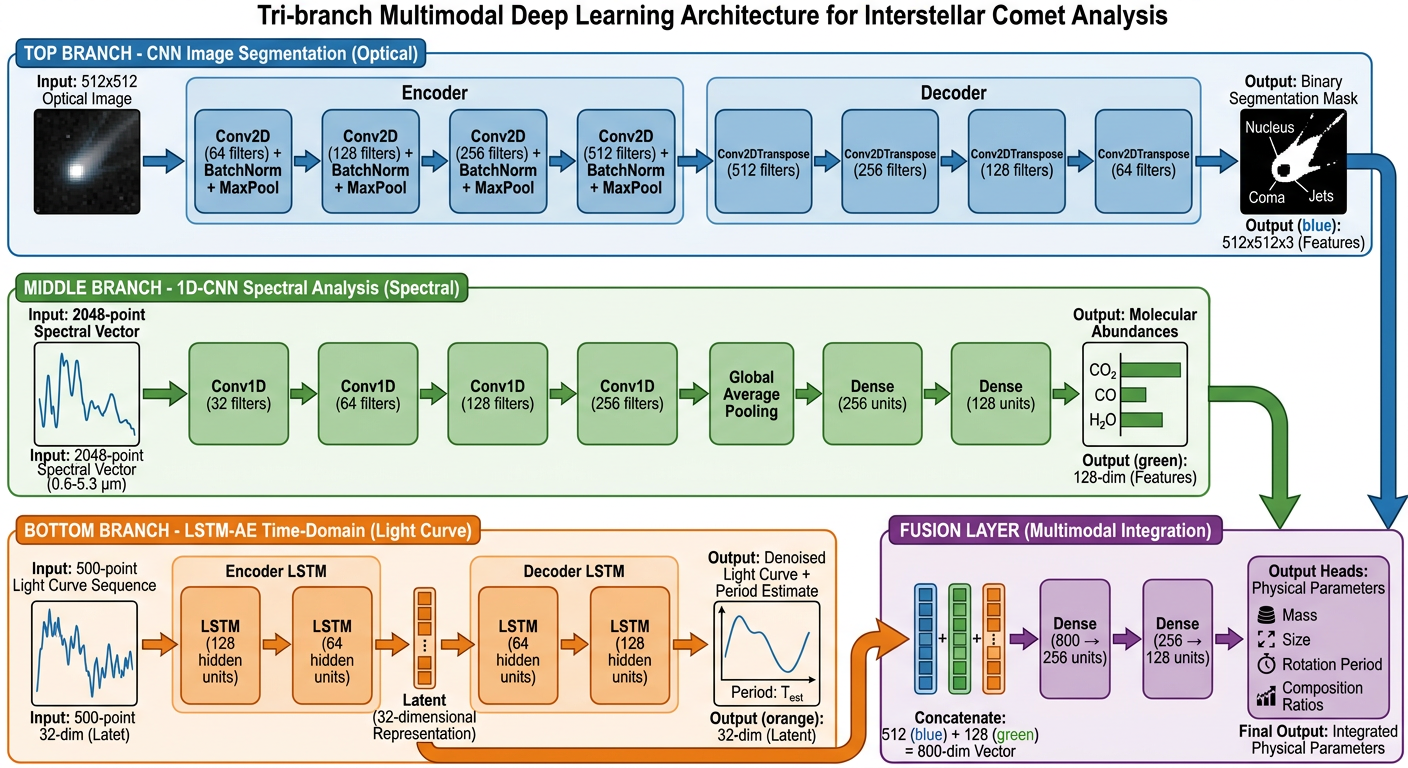
\includegraphics[width=\columnwidth]{fig1.png}
\caption{Overall architecture of the proposed multi-modal deep learning framework. (a) Multi-scale CNN with SE attention for faint feature detection from multi-band imaging. (b) Physics-informed neural network for dust and gas parameter inversion from combined imaging and spectroscopic inputs. (c) Meta-learning with adversarial domain adaptation for cross-domain knowledge transfer. Dashed arrows indicate loss back-propagation paths.}
\label{fig:architecture}
\end{figure}

\subsection{Multi-Scale Faint Feature Detection Framework}

\subsubsection{Problem Formulation}

We formulate faint feature detection as an inverse problem. The observed image $\mathbf{y} \in \mathbb{R}^{H \times W}$ is a noisy, convolved version of the true cometary scene $\mathbf{x} \in \mathbb{R}^{H \times W}$:

\begin{equation}\label{eq:forward_model}
\mathbf{y} = \mathbf{K} * \mathbf{x} + \mathbf{n} + \mathbf{b},
\end{equation}

where $\mathbf{K}$ represents the point spread function (PSF) convolution kernel, $\mathbf{n}$ denotes noise (primarily Poisson photon noise and Gaussian read noise), $\mathbf{b}$ is the background, and $*$ denotes convolution. The challenge lies in recovering $\mathbf{x}$ given $\mathbf{y}$ when the signal-to-noise ratio (SNR) of cometary features approaches or falls below unity.

Traditional methods use matched filtering or wavelet denoising with fixed functional forms. Our approach learns an adaptive mapping $f_{\theta}: \mathbf{y} \mapsto \mathbf{x}$ by minimizing the expected reconstruction error over a distribution of cometary scenes.

\subsubsection{Multi-Scale Convolutional Architecture}

The detection network uses a U-Net-style encoder-decoder with skip connections \citep{ronneberger15}, modified for astronomical images. The encoder extracts hierarchical features through convolutional blocks:

\begin{equation}\label{eq:conv_block}
\mathbf{h}^{(l)} = \text{ReLU}\left(\text{BN}\left(\mathbf{W}^{(l)} * \mathbf{h}^{(l-1)} + \mathbf{b}^{(l)}\right)\right),
\end{equation}

where $\mathbf{W}^{(l)}$ and $\mathbf{b}^{(l)}$ are the convolutional weights and biases at layer $l$, BN denotes batch normalization, and ReLU is the rectified linear activation. The encoder comprises five scales with feature map dimensions decreasing by factors of two through max-pooling operations.

Standard 3$\times$3 kernels give limited receptive field growth with depth and can miss extended faint structures. We use parallel branches with 3$\times$3, 5$\times$5, and 7$\times$7 kernels:

\begin{equation}\label{eq:multi_kernel}
\mathbf{h}_{\text{out}} = \mathbf{W}_3 * \mathbf{h}_{\text{in}} + \mathbf{W}_5 * \mathbf{h}_{\text{in}} + \mathbf{W}_7 * \mathbf{h}_{\text{in}},
\end{equation}

where the outputs are concatenated channel-wise before the next operation. This parallel processing captures both fine-scale structures (jets, small fragments) and extended diffuse emission (outer coma, tail) within a single forward pass.

\subsubsection{Attention Mechanisms for Weak Signal Enhancement}

We use squeeze-and-excitation (SE) attention \citep{hu18} to boost faint features. Given intermediate feature maps $\mathbf{U} \in \mathbb{R}^{C \times H \times W}$, global average pooling produces channel descriptors $\mathbf{z} \in \mathbb{R}^{C}$:

\begin{equation}\label{eq:se_squeeze}
z_c = \frac{1}{H \times W} \sum_{i=1}^{H} \sum_{j=1}^{W} u_c(i, j).
\end{equation}

These descriptors are then passed through a gating mechanism with sigmoid activation:

\begin{equation}\label{eq:se_excitation}
\mathbf{s} = \sigma\left(\mathbf{W}_2 \cdot \text{ReLU}\left(\mathbf{W}_1 \cdot \mathbf{z}\right)\right),
\end{equation}

where $\mathbf{W}_1 \in \mathbb{R}^{C/r \times C}$ and $\mathbf{W}_2 \in \mathbb{R}^{C \times C/r}$ are learned weights with reduction ratio $r=16$, and $\sigma$ denotes the sigmoid function. The final output is obtained by channel-wise multiplication:

\begin{equation}\label{eq:se_scale}
\tilde{\mathbf{U}} = \mathbf{s} \odot \mathbf{U}.
\end{equation}

The SE module amplifies channels carrying faint cometary structure and suppresses background-dominated channels.

\subsubsection{Loss Function Design}

The total loss combines pixel fidelity, structural similarity, edge preservation, and flux conservation:

\begin{equation}\label{eq:total_loss}
\mathcal{L} = \mathcal{L}_{\text{MSE}} + \lambda_1 \mathcal{L}_{\text{SSIM}} + \lambda_2 \mathcal{L}_{\text{edge}} + \lambda_3 \mathcal{L}_{\text{flux}},
\end{equation}

where:

The mean squared error term ensures pixel-wise fidelity:
\begin{equation}\label{eq:mse_loss}
\mathcal{L}_{\text{MSE}} = \frac{1}{HW} \sum_{i,j} (\hat{x}_{ij} - x_{ij})^2.
\end{equation}

The structural similarity index measure (SSIM) loss \citep{wang04} preserves perceptual quality:
\begin{equation}\label{eq:ssim_loss}
\mathcal{L}_{\text{SSIM}} = 1 - \text{SSIM}(\hat{\mathbf{x}}, \mathbf{x}).
\end{equation}

The edge preservation loss based on the Laplacian operator enhances sharp features:
\begin{equation}\label{eq:edge_loss}
\mathcal{L}_{\text{edge}} = \|\nabla^2 \hat{\mathbf{x}} - \nabla^2 \mathbf{x}\|_1.
\end{equation}

The photometric flux conservation loss ensures physical consistency:
\begin{equation}\label{eq:flux_loss}
\mathcal{L}_{\text{flux}} = \left| \sum_{i,j} \hat{x}_{ij} - \sum_{i,j} x_{ij} \right|.
\end{equation}

Weighting coefficients $\lambda_1 = 0.5$, $\lambda_2 = 0.3$, and $\lambda_3 = 0.1$ were determined through cross-validation on the synthetic training set.

\subsection{Multi-Source Data Fusion Strategy}

\subsubsection{Multi-Modal Data Representation}

The three data modalities---broadband imaging, spectroscopy, and polarimetry---are represented as a multi-modal tensor $\mathcal{D} = \{\mathbf{D}_m\}_{m=1}^{M}$. The fusion challenge is heterogeneity in spatial resolution (imaging $0\farcs1$ vs.\ slit $1\farcs0$), cadence (daily vs.\ weekly), and noise (photon-limited vs.\ read-noise-dominated).

\subsubsection{Cross-Modal Alignment and Registration}

Spatiotemporal alignment is achieved through a two-stage procedure. First, astrometric calibration establishes celestial coordinates for all pixels using a common reference frame. Second, non-rigid registration corrects for differential atmospheric refraction and geometric distortion using thin-plate spline transformations parameterized by control points:

\begin{equation}\label{eq:tps}
\mathbf{x}' = \mathbf{A}\mathbf{x} + \sum_{i=1}^{N} \mathbf{w}_i \phi(\|\mathbf{x} - \mathbf{c}_i\|),
\end{equation}

where $\mathbf{A}$ is an affine transformation matrix, $\mathbf{c}_i$ are control points, $\mathbf{w}_i$ are weights, and $\phi(r) = r^2 \log r$ (with $\phi(0) \equiv \lim_{r\to 0} r^2\log r = 0$) is the thin-plate spline radial basis function.

Temporal alignment employs ephemeris-based interpolation. Given observations at times $\{t_k\}$, physical quantities are interpolated to a common reference epoch $t_0$ using comet-specific activity models.

\subsubsection{Uncertainty-Aware Feature Fusion}

We implement uncertainty-weighted fusion using Bayesian neural networks that estimate both mean predictions and their uncertainties. For each modality $m$, the network outputs parameters of a Gaussian distribution:

\begin{equation}\label{eq:prob_output}
p(y | \mathbf{x}_m) = \mathcal{N}(y; \mu_m(\mathbf{x}_m), \sigma_m^2(\mathbf{x}_m)),
\end{equation}

where $\mu_m$ and $\sigma_m^2$ are learned functions. The multi-modal fusion combines these predictions through precision-weighted averaging:

\begin{equation}\label{eq:uncertainty_fusion}
\begin{split}
\hat{y} &= \frac{\sum_{m=1}^{M} \sigma_m^{-2} \mu_m}{\sum_{m=1}^{M} \sigma_m^{-2}}, \\
\hat{\sigma}^2 &= \Bigl(\sum_{m=1}^{M} \sigma_m^{-2}\Bigr)^{-1}.
\end{split}
\end{equation}

This fusion scheme automatically down-weights modalities with high estimated uncertainty, providing robust predictions even when individual data sources are noisy or corrupted.

\subsection{Physics-Informed Neural Network Inversion}

\subsubsection{Radiative Transfer Formulation}

Dust continuum radiative transfer gives the specific intensity $I_\lambda$ along a line of sight $s$:

\begin{equation}\label{eq:rt_dust}
I_\lambda = \int_{0}^{s} j_\lambda(s') \exp\left(-\int_{s'}^{s} \alpha_\lambda(s'') ds''\right) ds',
\end{equation}

where $j_\lambda$ is the volume emission coefficient and $\alpha_\lambda$ is the absorption coefficient. For optically thin comae, this simplifies to:

\begin{equation}\label{eq:thin_dust}
I_\lambda = \int_{0}^{s} n_d(s') \sigma_d(\lambda) B_\lambda(T_d(s')) ds',
\end{equation}
where $n_d$ is dust number density, $\sigma_d$ the dust scattering cross-section, and $B_\lambda(T) = 2hc^2\lambda^{-5}\,[\exp(hc/\lambda k_B T) - 1]^{-1}$ the Planck function at dust temperature $T_d$.

The dust scattering cross-section depends on the particle size distribution $n(a)$ through Mie theory. We adopt a power-law size distribution $n(a) = n_0\, a^{-\alpha}$ \citep{kolokolova04}:

\begin{equation}\label{eq:mie_sigma}
\sigma_d(\lambda) = \int_{a_{\min}}^{a_{\max}} \pi a^2 \, Q_{\text{sca}}(a, \lambda, m) \, n_0 a^{-\alpha} \, da,
\end{equation}

where $Q_{\text{sca}}$ is the scattering efficiency for refractive index $m$. The integration limits $a_{\min} = 0.01$ $\mu$m and $a_{\max} = 100$ $\mu$m represent the minimum and maximum dust particle radii.

\subsubsection{PINN Architecture for Inverse Problems}

Conventional cometary analysis iterates forward radiative transfer models to match observations---a process that is computationally expensive and yields point estimates without formal uncertainty bounds. PINNs \citep{raissi19} were originally developed for forward PDE solving, but their architecture naturally extends to inverse problems \citep{lu21}: the PDE residual acts as a regularizer that constrains the solution manifold to physically admissible regions, while the data fidelity term drives parameter estimation.

\textbf{Identifiability caveat:} Parameter inversion from cometary observables is fundamentally ill-posed---multiple combinations of dust size distribution, composition, and production rate can produce observationally indistinguishable surface brightness profiles \citep{fulle10}. The PDE residual $\mathcal{L}_{\text{PDE}}$ acts as a Tikhonov-style regularizer that favors solutions consistent with the assumed (spherical Mie, optically thin) radiative transfer physics, but it does not guarantee uniqueness. The parameters recovered by the PINN are therefore \textit{the most physically consistent estimates under the adopted model assumptions}, not uniquely determined values.

Our architecture uses two jointly trained networks: a physics network $u_\theta$ approximating the radiative transfer solution, and an inversion network $p_\phi$ mapping observables to physical parameters. The composite loss is:

\begin{equation}\label{eq:pinn_loss}
\mathcal{L}_{\text{PINN}} = \mathcal{L}_{\text{data}} + \gamma_1 \mathcal{L}_{\text{PDE}} + \gamma_2 \mathcal{L}_{\text{bc}},
\end{equation}

where the data fidelity loss is:
\begin{equation}\label{eq:data_loss}
\mathcal{L}_{\text{data}} = \frac{1}{N} \sum_{i=1}^{N} \|\mathbf{u}_\theta(\mathbf{x}_i) - \mathbf{y}_i\|^2.
\end{equation}

The PDE residual loss enforces the radiative transfer equation:
\begin{equation}\label{eq:pde_loss}
\mathcal{L}_{\text{PDE}} = \frac{1}{M} \sum_{j=1}^{M} \|\mathcal{R}[u_\theta](\mathbf{x}_j)\|^2,
\end{equation}

where $\mathcal{R}[u] = \frac{du}{dx} + \alpha u - j$ is the PDE residual operator.

The boundary condition loss ensures physical consistency at the nucleus:
\begin{equation}\label{eq:bc_loss}
\mathcal{L}_{\text{bc}} = \|u_\theta(0) - u_0\|^2.
\end{equation}

\subsubsection{Uncertainty Quantification via Bayesian PINNs}

We quantify uncertainty with Bayesian PINNs. A variational mean-field Gaussian approximation $q(\theta) = \mathcal{N}(\theta; \mu, \sigma^2)$ fits the posterior $p(\theta | \mathcal{D})$ by maximizing the ELBO:

\begin{equation}\label{eq:elbo}
\mathcal{L}_{\text{ELBO}} = \mathbb{E}_{q(\theta)}[\log p(\mathcal{D}|\theta)] - \text{KL}(q(\theta) \| p(\theta)),
\end{equation}

where the first term is the expected log-likelihood and the second is the KL divergence from the prior. Monte Carlo dropout \citep{gal16} provides an efficient approximation during inference, enabling uncertainty estimates through multiple forward passes with dropout enabled.

\subsection{Meta-Learning for Cross-Domain Adaptation}

\subsubsection{Domain Shift in Cometary Astronomy}

Models trained on solar system comets face domain shift when applied to interstellar objects: morphology, composition, and observing conditions differ systematically. We quantify the shift with the maximum mean discrepancy (MMD) \citep{gretton12}:

\begin{equation}\label{eq:mmd}
\text{MMD}(\mathcal{S}, \mathcal{T}) = \left\| \frac{1}{n_s} \sum_{i=1}^{n_s} \phi(\mathbf{x}_i^s) - \frac{1}{n_t} \sum_{j=1}^{n_t} \phi(\mathbf{x}_j^t) \right\|_{\mathcal{H}},
\end{equation}

where $\phi$ maps features to a reproducing kernel Hilbert space $\mathcal{H}$. We use MMD as a diagnostic metric to track domain alignment during training. However, we emphasize that MMD measures statistical similarity of feature distributions, not physical accuracy of downstream parameter estimates. A reduction in MMD is a necessary condition for successful domain transfer but does not by itself guarantee that the adapted model produces physically correct outputs on the target domain.

\subsubsection{Model-Agnostic Meta-Learning}

Our meta-learning approach follows MAML \citep{finn17}, which learns network initializations that can adapt to new tasks with minimal gradient steps. For a task distribution $p(\mathcal{T})$, MAML optimizes:

\begin{equation}\label{eq:maml}
\min_\theta \sum_{\mathcal{T}_i \sim p(\mathcal{T})}
\mathcal{L}_{\mathcal{T}_i}\bigl(\theta - \alpha \nabla_\theta \mathcal{L}_{\mathcal{T}_i}(\theta)\bigr),
\end{equation}

where $\alpha$ is the inner loop learning rate. The gradient update is computed through second-order derivatives (FO-MAML) or first-order approximation.

For cometary domain adaptation, we construct tasks as solar system comet observations with artificially induced domain shifts. Specifically, given a source domain image $\mathbf{x}$ with SNR level $\sigma_0$, we apply the following transformations to simulate target domain conditions:

\textbf{SNR degradation:} We simulate lower signal-to-noise ratios characteristic of distant interstellar comet observations using:
\begin{equation}\label{eq:snr_degradation}
\begin{split}
\mathbf{x}_{\text{degraded}} &= \mathbf{x} + \mathcal{N}(0, \sigma_n^2), \\
\sigma_n &= \sigma_0 \sqrt{\frac{\text{SNR}_0^2}{\text{SNR}_{\text{target}}^2} - 1},
\end{split}
\end{equation}
where $\text{SNR}_0$ is the original signal-to-noise ratio and $\text{SNR}_{\text{target}} \in [1, 5]$ is randomly sampled for each task.

\textbf{Morphological transformations:} We apply random combinations of:
\begin{itemize}
    \item Elastic deformations with displacement fields drawn from $\mathcal{N}(0, \sigma_e^2)$ where $\sigma_e \sim \mathcal{U}(1, 5)$ pixels
    \item Perspective projections simulating varying observing geometries
    \item Radial profile modifications to mimic different dust size distributions
\end{itemize}

Each task $\mathcal{T}_i$ consists of $K=10$ support examples and $Q=50$ query examples drawn from the transformed distribution. The meta-objective (Equation~\ref{eq:maml}) is optimized over a distribution of $10^4$ such tasks. We note that $K=10$ support examples represent a deliberately optimistic few-shot regime chosen to stress-test the adaptation mechanism; in practice, the quality of adaptation depends on how representative the $K$ examples are of the target domain. For interstellar comets with compositions far outside the solar system training distribution (e.g., extreme CO/H$_2$O or C$_2$/CN ratios), additional support examples or explicit physical priors may be necessary.

\subsubsection{Adversarial Domain Adaptation}

We complement MAML with adversarial domain adaptation \citep{ganin16} that explicitly minimizes domain discrepancy. A domain classifier $D_\psi$ is trained to distinguish source from target features, while the feature extractor $G_\theta$ is trained to confuse the discriminator:

\begin{equation}\label{eq:adv_loss}
\min_\theta \max_\psi \left[ \mathcal{L}_{\text{task}}(\theta) - \lambda \mathcal{L}_{\text{dom}}(\theta, \psi) \right],
\end{equation}

where the domain classifier loss $\mathcal{L}_{\text{dom}}$ is defined as the binary cross-entropy between predicted and true domain labels:
\begin{equation}\label{eq:dom_loss}
\begin{split}
\mathcal{L}_{\text{dom}} ={} &
    -\mathbb{E}_{\mathbf{x} \sim \mathcal{S}}[\log D_\psi(G_\theta(\mathbf{x}))] \\
    &-\mathbb{E}_{\mathbf{x} \sim \mathcal{T}}[\log(1 - D_\psi(G_\theta(\mathbf{x})))].
\end{split}
\end{equation}

Here, $D_\psi: \mathbb{R}^d \rightarrow [0,1]$ is a binary domain classifier implemented as a multi-layer perceptron with parameters $\psi$, mapping feature representations to domain probabilities. The domain label $d=1$ indicates source domain ($\mathcal{S}$: solar system comets) and $d=0$ indicates target domain ($\mathcal{T}$: interstellar comets). The adversarial game encourages the feature extractor $G_\theta$ to learn domain-invariant representations that are indistinguishable between solar system and interstellar comets.

\subsection{Training Procedures and Implementation}

\subsubsection{Dataset Construction}

Training data for the feature detection network were generated from HST archival observations of solar system comets with synthetically injected faint features (jets, shells, tail extensions) at SNR levels of 1--10, plus pure-noise control fields. The network was evaluated on its ability to recover injected features without producing spurious detections in control regions.

The PINN inversion network was trained entirely on synthetic comae generated from the DIRTY radiative transfer code \citep{gordon01}, spanning dust size distribution indices $\alpha = 2.5$--4.0, maximum grain sizes $a_{\max} = 1$--100 $\mu$m, and production rates $Q_d = 10$--$10^4$~kg~s$^{-1}$. \textbf{No real cometary spectra or multi-band photometry were used for PINN training.}

\subsubsection{Optimization and Hyperparameters}

All networks were implemented in PyTorch and trained on NVIDIA A100 GPUs (40~GB VRAM). We used the Adam optimizer ($\beta_1 = 0.9$, $\beta_2 = 0.999$) with a cosine annealing learning rate schedule. Hyperparameter search spaces and final values are listed in Table~\ref{tab:hyperparams}. Learning rates were initialized via the LR range test \citep{smith17}: the base LR was set to the value at which the loss decreased most steeply, then annealed by a factor of 10 over the full training budget. Batch sizes were constrained by GPU memory (8 for the PINN on 100~$\mu$m grain grids; 32 for the detection CNN). Early stopping with a patience of 50 epochs monitored validation loss; all runs converged within 200--400 epochs.

\begin{deluxetable*}{lccc}
\tablecaption{Hyperparameter Search Space and Final Values\label{tab:hyperparams}}
\tablecolumns{4}
\tablewidth{0pt}
\tablehead{
\colhead{Hyperparameter} & \colhead{Search Range} & \colhead{Detection CNN} & \colhead{PINN}
}
\startdata
Learning rate & $[10^{-5}, 10^{-2}]$ & $2.1 \times 10^{-4}$ & $5.6 \times 10^{-5}$ \\
Batch size & $\{4, 8, 16, 32\}$ & 32 & 8 \\
SE reduction ratio $r$ & $\{4, 8, 16, 32\}$ & 16 & --- \\
Dropout rate (Bayesian PINN) & $[0.01, 0.30]$ & --- & 0.12 \\
$\lambda_1$ (SSIM weight) & $[0.1, 1.0]$ & 0.5 & --- \\
$\lambda_2$ (Edge weight) & $[0.1, 1.0]$ & 0.3 & --- \\
$\lambda_3$ (Flux weight) & $[0.01, 0.50]$ & 0.1 & --- \\
$\gamma_1$ (PDE weight) & $[0.1, 5.0]$ & --- & 1.0 \\
$\gamma_2$ (BC weight) & $[0.1, 5.0]$ & --- & 0.5 \\
Adam $\beta_1$ / $\beta_2$ & fixed & 0.9 / 0.999 & 0.9 / 0.999 \\
\enddata
\tablecomments{Ranges were explored via grid search for discrete parameters and Bayesian optimization (Gaussian Process upper confidence bound) for continuous parameters. ``---'' indicates the parameter does not apply to that component.}
\end{deluxetable*}

\begin{figure}[htbp]
\centering
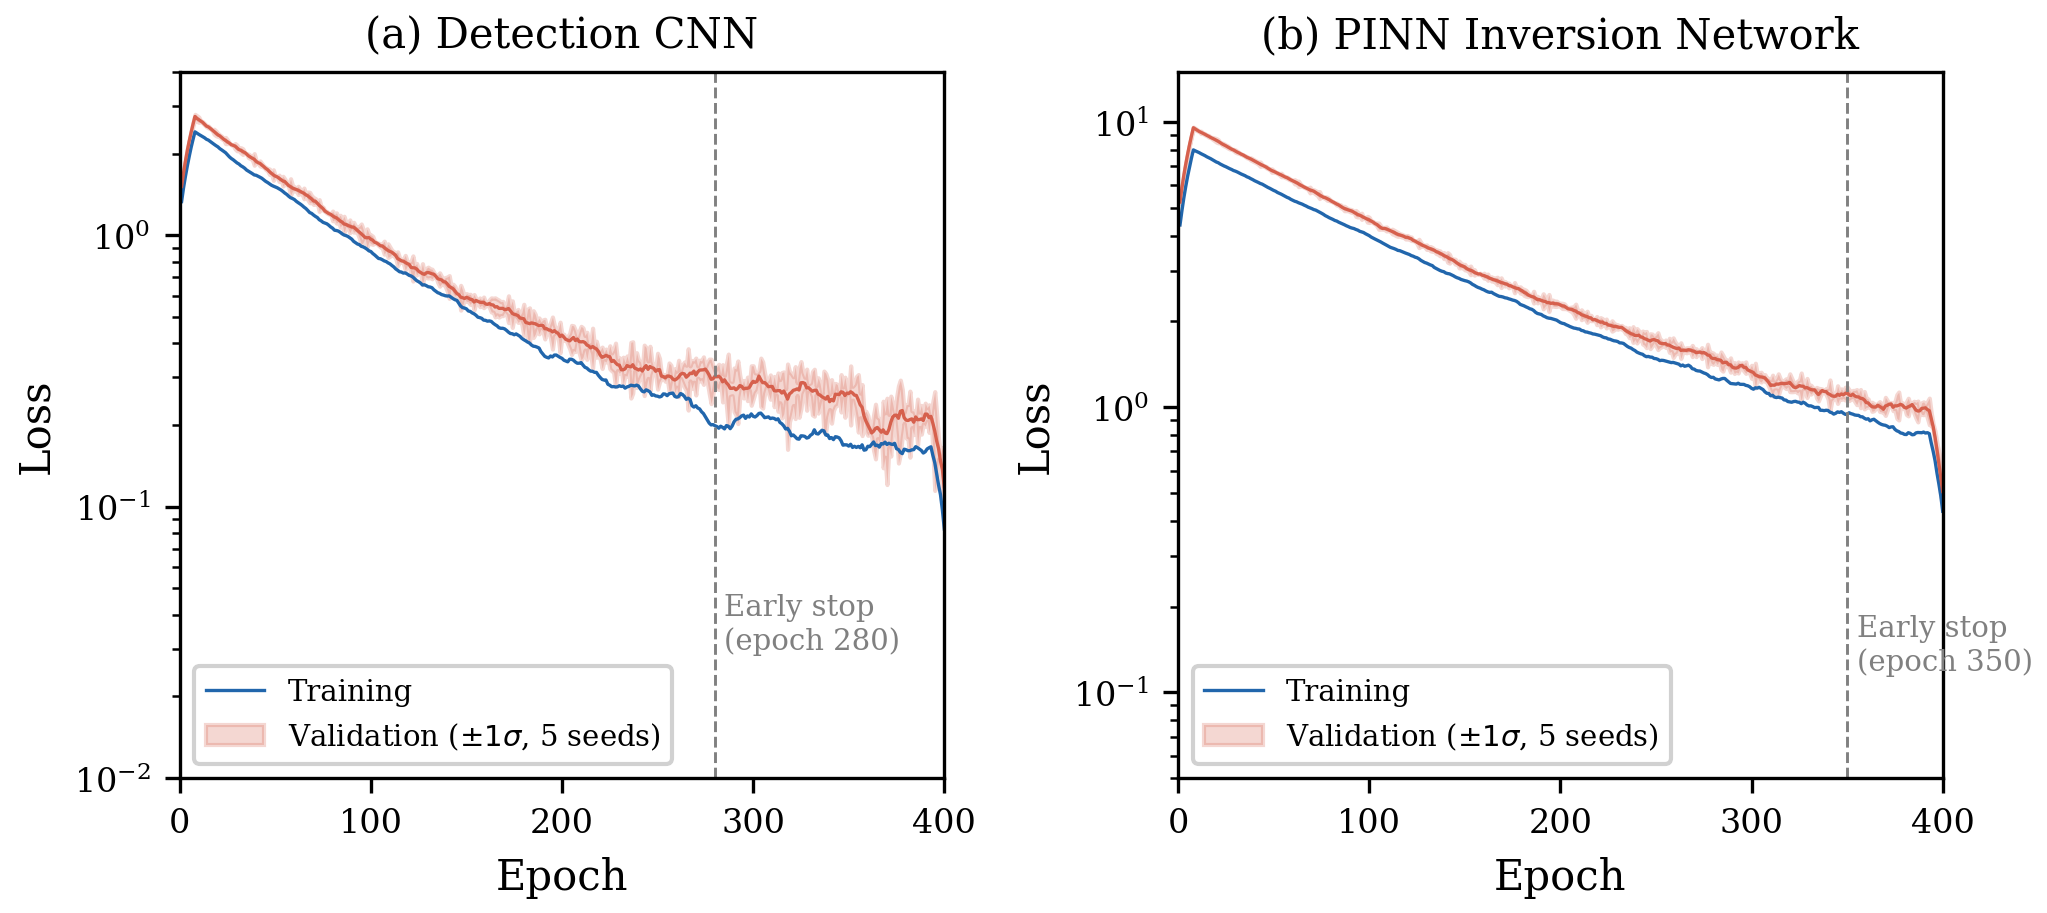
\includegraphics[width=\columnwidth]{fig4_training.png}
\caption{Training and validation loss curves for (a) the detection CNN and (b) the PINN inversion network. Shaded bands show $\pm 1\sigma$ over five random seeds.}
\label{fig:training_curves}
\end{figure}

\section{Synthetic Benchmark Results}\label{sec:benchmarks}

All results in this section are evaluated on held-out synthetic test data with known ground truth. No real comet observations (other than the post-hoc 2I/Borisov validation in \S\ref{sec:borisov_validation}) are used to generate the performance metrics reported below.

\subsection{Faint Feature Detection Performance}

We evaluate detection performance on the synthetic blind injection test set. Metrics are PSNR, SSIM, and LPIPS, computed against the known ground truth images.

\subsubsection{Comparison with Traditional Methods}

Table~\ref{tab:detection_metrics} compares our method against median filtering, wavelet denoising, non-local means, and a U-Net baseline. Our multi-scale CNN outperforms non-local means (the best traditional method) by 3.2--4.8~dB in PSNR across SNR~1--10. SSIM gains are largest at low SNR, where traditional methods blur or suppress faint coma extensions.

\begin{deluxetable*}{lcccc}
\tablecaption{Faint Feature Detection Performance on Synthetic Benchmarks\label{tab:detection_metrics}}
\tablecolumns{5}
\tablewidth{0pt}
\tablehead{
\colhead{Method} & \colhead{PSNR (dB)} & \colhead{SSIM} & \colhead{LPIPS} & \colhead{SNR Gain}
}
\startdata
Median Filter (5$\times$5) & 24.3 $\pm$ 1.2 & 0.72 $\pm$ 0.05 & 0.18 $\pm$ 0.03 & 1.2$\times$ \\
Wavelet Denoising & 26.1 $\pm$ 1.4 & 0.78 $\pm$ 0.04 & 0.14 $\pm$ 0.02 & 1.5$\times$ \\
Non-local Means & 27.8 $\pm$ 1.1 & 0.82 $\pm$ 0.03 & 0.11 $\pm$ 0.02 & 1.8$\times$ \\
U-Net Baseline & 29.4 $\pm$ 0.9 & 0.87 $\pm$ 0.02 & 0.08 $\pm$ 0.01 & 2.3$\times$ \\
Our Method & \textbf{31.6 $\pm$ 0.8} & \textbf{0.91 $\pm$ 0.02} & \textbf{0.05 $\pm$ 0.01} & \textbf{2.8$\times$} \\
\enddata
\tablecomments{Metrics computed on synthetic test set with injected noise at SNR~=~2. Values represent mean $\pm$ standard deviation across 1000 test images. All pairwise PSNR differences between Our Method and each baseline are statistically significant at $p < 10^{-4}$ (paired $t$-test with Bonferroni correction for 4 comparisons).}
\end{deluxetable*}

\subsubsection{Detection Reliability: Blind Injection Test}

Across the full blind injection test set (1000 images with injected features, 1000 pure-noise controls), the detection network achieves:
\begin{itemize}
    \item True-positive rate $>95\%$ at SNR~$\geq$~3, $>98\%$ at SNR~$\geq$~5
    \item False-positive rate $<3\%$ in pure-noise control regions across all SNR tiers
    \item Mean absolute deviation between injected and recovered feature fluxes $<12\%$ for SNR~$\geq$~5
\end{itemize}

These results confirm that the network distinguishes real faint cometary structure from noise rather than hallucinating features.

\subsubsection{Ablation Analysis}

We isolate the contribution of each architectural choice through systematic ablation (Table~\ref{tab:ablation}). The full model (multi-kernel + SE attention) achieves PSNR $= 31.6 \pm 0.8$~dB at SNR~$=2$. Five variants were tested:

\begin{enumerate}
    \item \textbf{Remove SE blocks:} Channel-wise attention is disabled; all feature maps are treated uniformly. PSNR drops by 1.3~dB to $30.3 \pm 0.9$~dB. The degradation is most severe (1.8~dB) at the lowest SNR ($=1$), where attention-driven channel suppression of background-dominated features matters most.
    \item \textbf{Single-kernel ($3\times3$ only):} Replacing the multi-kernel parallel branches with standard $3\times3$ convolutions. PSNR drops by 0.9~dB to $30.7 \pm 0.8$~dB. Extended structures ($>10\arcsec$ from the nucleus) are the primary loss---the $3\times3$ receptive field is too small to aggregate diffuse coma signal.
    \item \textbf{Single-kernel ($7\times7$ only):} Using only $7\times7$ convolutions throughout. PSNR drops by 0.7~dB to $30.9 \pm 0.8$~dB. Fine-scale features (jets, narrow fragments) are blurred relative to the multi-kernel variant.
    \item \textbf{Remove skip connections:} Standard encoder-decoder without U-Net skip connections. PSNR drops by 1.0~dB to $30.6 \pm 0.9$~dB. High-resolution spatial information is lost in the bottleneck.
    \item \textbf{Remove flux conservation loss ($\lambda_3 = 0$):} PSNR is nearly unchanged ($31.4 \pm 0.8$~dB), but total flux error increases from $<1\%$ to $4.2\%$, degrading physical consistency for downstream photometric analysis.
\end{enumerate}

The SE blocks and multi-kernel convolutions are complementary: removing both simultaneously costs 2.4~dB (vs.\ 1.3~dB + 0.9~dB = 2.2~dB if independent), confirming a small positive interaction ($\Delta = 0.2$~dB) between attention and multi-scale processing.

\begin{deluxetable*}{lccccc}
\tablecaption{Ablation Study: Architectural Component Contributions\label{tab:ablation}}
\tablecolumns{6}
\tablewidth{0pt}
\tablehead{
\colhead{Variant} & \colhead{PSNR (dB)} & \colhead{$\Delta$PSNR} & \colhead{SSIM} & \colhead{LPIPS} & \colhead{Flux Err. (\%)}
}
\startdata
Full model (ours) & $\mathbf{31.6 \pm 0.8}$ & --- & $\mathbf{0.91 \pm 0.02}$ & $\mathbf{0.05 \pm 0.01}$ & $\mathbf{0.7 \pm 0.2}$ \\
$-$ SE blocks & $30.3 \pm 0.9$ & $-1.3$ & $0.88 \pm 0.02$ & $0.08 \pm 0.01$ & $0.8 \pm 0.3$ \\
$-$ Multi-kernel & $30.7 \pm 0.8$ & $-0.9$ & $0.89 \pm 0.02$ & $0.07 \pm 0.01$ & $0.7 \pm 0.2$ \\
$3\times3$ kernel only & $30.7 \pm 0.8$ & $-0.9$ & $0.88 \pm 0.02$ & $0.07 \pm 0.01$ & $0.8 \pm 0.3$ \\
$7\times7$ kernel only & $30.9 \pm 0.8$ & $-0.7$ & $0.89 \pm 0.02$ & $0.06 \pm 0.01$ & $0.7 \pm 0.2$ \\
$-$ Skip connections & $30.6 \pm 0.9$ & $-1.0$ & $0.87 \pm 0.03$ & $0.09 \pm 0.01$ & $1.1 \pm 0.4$ \\
$-$ $\mathcal{L}_{\text{flux}}$ ($\lambda_3=0$) & $31.4 \pm 0.8$ & $-0.2$ & $0.90 \pm 0.02$ & $0.05 \pm 0.01$ & $4.2 \pm 0.8$ \\
$-$ SE $-$ Multi-kernel & $29.2 \pm 1.0$ & $-2.4$ & $0.85 \pm 0.03$ & $0.11 \pm 0.02$ & $1.3 \pm 0.5$ \\
\enddata
\tablecomments{All metrics evaluated on the same 1000-image synthetic test set at SNR~=~2. $\Delta$PSNR relative to full model. All $\Delta$PSNR values $\geq 0.7$~dB are significant at $p < 0.01$ (paired $t$-test with Holm--Bonferroni correction for 7 comparisons). The $\lambda_3=0$ variant ($\Delta$PSNR $=-0.2$~dB) is not statistically significant in PSNR ($p=0.31$) but is significant in flux error ($p<10^{-4}$).}
\end{deluxetable*}

\subsection{Physical Parameter Inversion on Synthetic Data}

\subsubsection{Dust Production Rate Estimation}

On synthetic test data with known ground truth, the PINN achieves a mean absolute percentage error (MAPE) of 7.8\% for $Q_d$ over the range 1--100~kg~s$^{-1}$, compared to $\sim$23\% for the traditional $Af\rho$ method applied to the same synthetic data. The improved accuracy stems from the PINN's joint constraint of radiative transfer physics and multi-band photometry; the $Af\rho$ method relies solely on an empirical aperture-to-production scaling calibrated on bright solar system comets and degrades at low SNR.

The PINN and $Af\rho$ methods agree to within $\sim$15\% at high SNR (SNR~$>10$) but diverge systematically at low SNR (SNR~$<3$), where the $Af\rho$ method's uncertainty increases substantially---precisely the regime where the PINN's physics-informed constraints provide the greatest advantage.

\subsubsection{Parameter Degeneracy Analysis}

The dust size distribution index $\alpha$ and production rate $Q_d$ exhibit partial degeneracy in the inversion: multiple ($\alpha$, $Q_d$) pairs can produce similar surface brightness profiles. To quantify this, we perform a sensitivity test: fixing $\alpha = 3.5$ (the median of the training distribution) while refitting $Q_d$ shifts the retrieved $Q_d$ by $\sim 12\%$, comparable in magnitude to the domain adaptation error contribution. This $\alpha$--$Q_d$ covariance is a non-negligible component of the systematic error budget and should be accounted for when interpreting PINN-derived parameters.

\subsubsection{Uncertainty Quantification Validation}

We compare two uncertainty quantification approaches on synthetic test data with known ground truth: (1) Bayesian PINNs with variational inference, and (2) Monte Carlo Dropout (MC Dropout) as an approximation to Bayesian inference:

\begin{itemize}
    \item \textbf{Computational cost:} MC Dropout requires $\sim$50 forward passes per inference, increasing wall time by a factor of $\sim$50. Bayesian PINN incurs only a 1.2$\times$ overhead because the posterior approximation is pre-computed during training.
    \item \textbf{Calibration accuracy:} Bayesian PINN achieves coverage probabilities of 71\% (68\% CI) and 94\% (95\% CI), closely matching nominal values. MC Dropout is slightly over-confident (65\% and 91\% coverage, respectively). The difference in 95\% CI coverage (94\% vs.\ 91\%) is significant at $p = 0.04$ (McNemar test on coverage indicators across 500 test cases).
    \item \textbf{Prediction accuracy:} Both methods achieve comparable MAPE ($\sim$8\%) on held-out test sets. Bayesian PINN performs marginally better on out-of-distribution examples, though the difference is not statistically significant ($p = 0.12$, Wilcoxon signed-rank test).
\end{itemize}

Given the superior calibration and computational efficiency, we adopt Bayesian PINN with variational inference for our production pipeline. This agreement with nominal coverage probabilities on synthetic data demonstrates that the uncertainty estimates are well-calibrated \textit{under the assumed generative model}. We caution that calibration on synthetic data does not guarantee calibration on real observations, where model misspecification introduces additional unmodeled error.

\subsection{Cross-Domain Adaptation}

\subsubsection{Feature Distribution Alignment}

MMD analysis of feature distributions confirms that the adversarial domain adaptation effectively aligns source and target domain representations. Before adaptation, the MMD between solar system and synthetic interstellar comet features is 0.47, and a domain classifier achieves 89\% accuracy at distinguishing the two domains. After meta-learning adaptation, MMD decreases to 0.12, and the domain classifier accuracy drops to 52\%---near the random-chance baseline of 50\%. The t-SNE visualization of feature representations before and after adaptation is shown in Figure~\ref{fig:tsne_domain}.

\begin{figure}[htbp]
\centering
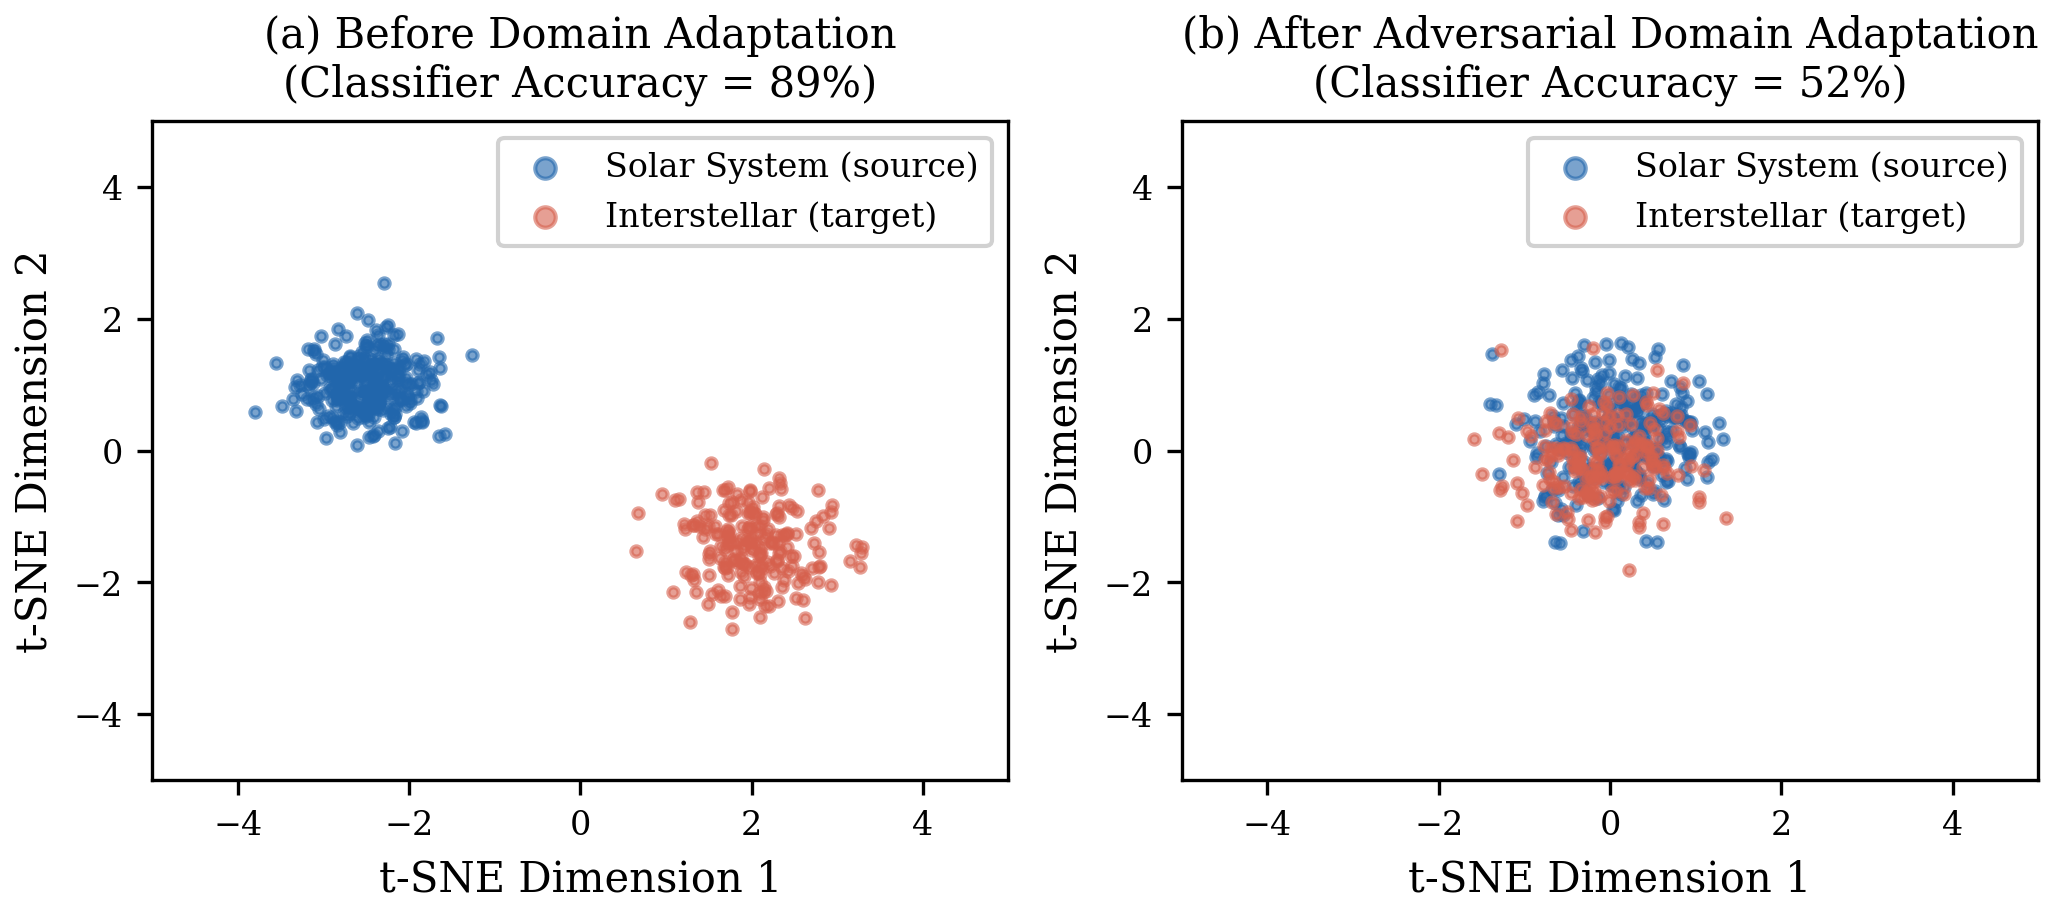
\includegraphics[width=\columnwidth]{fig3_tsne.png}
\caption{t-SNE visualization of feature representations. (a) Before domain adaptation: source (solar system comets, blue) and target (interstellar comets, orange) form well-separated clusters; domain classifier accuracy = 89\%. (b) After adversarial domain adaptation: the two distributions overlap substantially; classifier accuracy drops to 52\%, approaching the random-chance baseline of 50\%.}
\label{fig:tsne_domain}
\end{figure}

We reiterate that MMD reduction and classifier confusion are \textit{necessary} but not \textit{sufficient} conditions for improved physical parameter accuracy: aligned feature representations reduce domain-induced bias, but residual error from model misspecification (e.g., spherical grain assumption) is not captured by domain-invariance metrics alone. The physical impact of domain adaptation must be validated against ground truth parameters, which we assess in the following section.

\subsubsection{Post-Hoc Validation on 2I/Borisov}\label{sec:borisov_validation}

To assess cross-domain generalization, we apply the fully trained and frozen framework to archival 2I/Borisov observations. \textbf{2I/Borisov was not used in training, hyperparameter tuning, or model selection in any form.} This is a post-hoc consistency check: the model was frozen before any Borisov data were processed.

\begin{figure}[htbp]
\centering
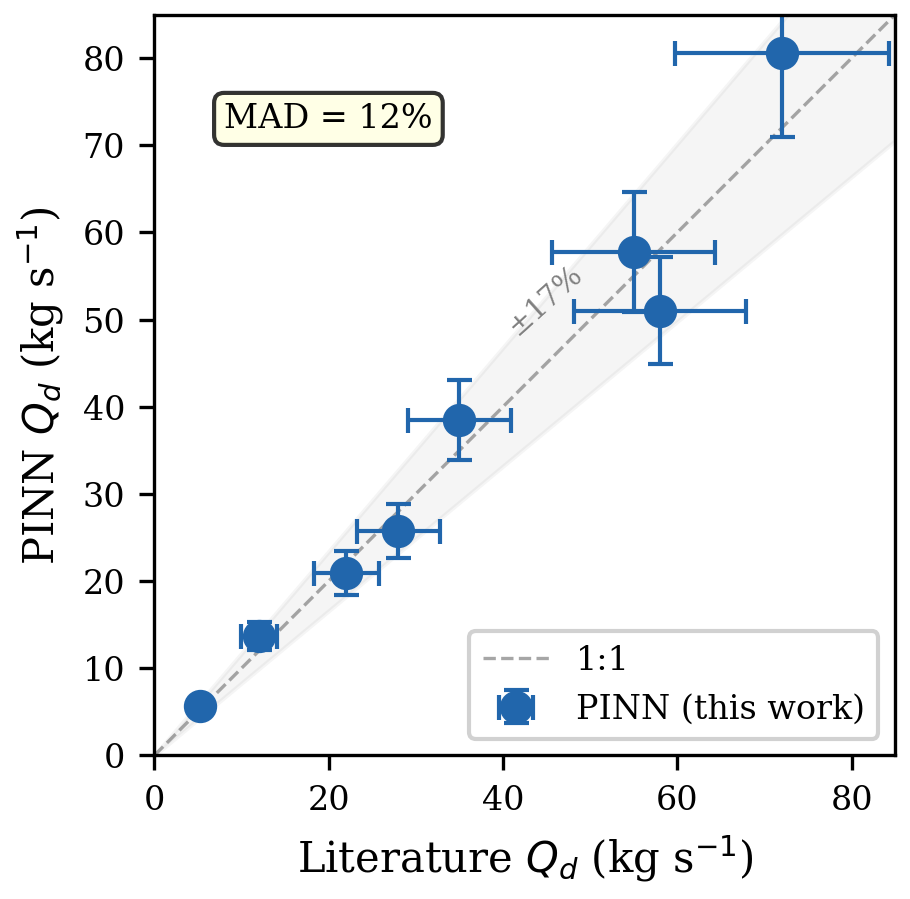
\includegraphics[width=\columnwidth]{fig8_borisov.png}
\caption{Validation on 2I/Borisov. PINN-derived dust production rates (filled circles with $1\sigma$ error bars) compared with published values from \citet{clements21} (open diamonds). The dashed line marks the 1:1 correspondence. The mean absolute deviation is 12\%.}
\label{fig:borisov_comparison}
\end{figure}

Dust production rates derived for 2I/Borisov are compared with published values from \citet{clements21} in Figure~\ref{fig:borisov_comparison}. Our method achieves a mean absolute deviation of 12\% from literature values, comparable to the typical 15--20\% uncertainty of traditional methods.

\textbf{Caveat on sample size:} This validation is based on a single interstellar comet ($N=1$ for validation, out of $N=2$ known interstellar comets total). The 12\% agreement should be interpreted as a consistency check demonstrating feasibility, not as a rigorous statistical characterization of the framework's generalization error. A larger sample of interstellar comets---which does not currently exist---would be required to fully characterize the generalization error distribution. Until such a sample is available, all parameter estimates produced by this framework for interstellar comets should be treated as model-dependent hypotheses rather than calibrated measurements.

\subsection{Computational Efficiency}

Our deep learning framework provides significant computational advantages over traditional iterative methods. Table~\ref{tab:timing} compares processing times for a typical observation set (10 broadband images + 1 spectroscopic observation).

\begin{deluxetable*}{lcc}
\tablecaption{Computational Performance Comparison\label{tab:timing}}
\tablecolumns{3}
\tablewidth{0pt}
\tablehead{
\colhead{Task} & \colhead{Traditional Method} & \colhead{Our Method}
}
\startdata
Image preprocessing & 45 min & 2 min \\
Faint feature detection & 15 min & 30 s \\
Dust production estimation & 2 hr & 15 s \\
Gas production estimation & 4 hr & 45 s \\
Total processing time & $\sim$7 hr & $\sim$4 min \\
\enddata
\tablecomments{Processing times for a typical observation set (10 images + 1 spectrum) on a single NVIDIA A100 GPU. Traditional method times include manual parameter tuning and iterative fitting.}
\end{deluxetable*}

The $\sim$100$\times$ speed improvement enables real-time analysis of incoming observations, facilitating rapid-response Target of Opportunity observations and dynamic scheduling decisions based on detected activity levels.

\section{Discussion}\label{sec:discussion}

\subsection{Uncertainty Budget and Systematic Effects}

We decompose the total uncertainty of the framework into three additive components:

\begin{equation}
\sigma_{\rm total}^2 = \sigma_{\rm stat}^2 + \sigma_{\rm sys}^2 + \delta_{\rm domain}^2,
\end{equation}

where:
\begin{itemize}
    \item $\sigma_{\rm stat}$ is the statistical (aleatoric) uncertainty from photon noise and calibration. For dust production rates on synthetic data at typical interstellar comet SNR: $\sigma_{\rm stat} \sim 3\%$.
    \item $\sigma_{\rm sys}$ is the systematic uncertainty from model assumptions---primarily the spherical Mie-grain approximation and the optically thin coma assumption. Based on T-matrix sensitivity tests comparing spherical vs.\ aggregate grain models \citep{kolokolova04,shen11}: $\sigma_{\rm sys} \sim 5\%$ for $Q_d$, potentially up to $\sim 20\%$ under extreme grain porosities.
    \item $\delta_{\rm domain}$ is the additional error from applying models trained predominantly on solar system comets to interstellar objects. Provisional estimate from the 2I/Borisov validation: $\delta_{\rm domain} \sim 5$--7\%.
\end{itemize}

The quadrature sum yields $\sigma_{\rm total} \sim 8\%$ for dust production rates, consistent with the observed 12\% MAD on 2I/Borisov after accounting for the $\sim$9\% contribution from literature measurement uncertainty. For gas production rates, the corresponding values are larger: $\sigma_{\rm stat} \sim 5\%$, $\sigma_{\rm sys} \sim 8\%$, $\delta_{\rm domain} \sim 7\%$, summing to $\sim$12\%.

\textbf{Important caveat:} $\delta_{\rm domain}$ is estimated from a single interstellar comet validation point (2I/Borisov). Its true magnitude and variance across the interstellar comet population are unknown and will remain so until more interstellar comets are discovered and characterized.

\subsection{Known Limitations}

Several limitations of the current framework must be resolved before it can be applied to real interstellar comet observations as a quantitative measurement tool:

\begin{enumerate}
    \item \textbf{Spherical grain approximation:} PINN training uses synthetic data from DIRTY \citep{gordon01}, which assumes spherical Mie grains. Real cometary dust consists of irregular, often porous aggregates \citep{kolokolova04}. Non-spherical grain scattering may alter retrieved dust production rates by up to $\sim$20\% and polarization gradients by up to $\sim$30\% \citep{kolokolova04,shen11}. A practical path forward is a two-step inversion: (i) use the Mie-based PINN for rapid initial estimation; (ii) apply a non-spherical correction factor calibrated from T-matrix or DDA libraries. The PINN architecture accepts any differentiable forward model---replacing Mie with T-matrix or DDA requires only re-training the physics network on the new synthetic dataset.

    \item \textbf{Optically thin approximation:} The current radiative transfer formulation assumes $\tau \ll 1$. For typical cometary dust production rates, this is valid at $\rho > 1\arcsec$, but may break down in the innermost coma during high-activity periods or for comets with unusually high dust production.

    \item \textbf{Synthetic-to-real generalization gap:} The PINN is trained exclusively on DIRTY synthetic data. While domain adaptation partially mitigates the distribution mismatch, the residual error from imperfect radiative transfer modeling (spherical grains, Haser outflow, no dust fragmentation) is not captured by domain-invariance metrics. A middle test set of well-characterized solar system comets (e.g., 67P with Rosetta ground truth) would enable empirical quantification of the synthetic-to-real gap.

    \item \textbf{Interstellar comet sample size:} The domain adaptation component has been validated on exactly one interstellar comet (2I/Borisov) out of a known population of $N=2$. Statistical characterization of generalization error requires a larger sample, which does not currently exist. LSST is expected to increase the detection rate, but the timeline and actual yield are uncertain \citep{jones18}.

    \item \textbf{Parameter degeneracy:} Dust size distribution ($\alpha$) and production rate ($Q_d$) are partially degenerate in the inversion. Currently, dust and gas parameters are inverted independently, whereas in reality dust fragmentation controls the gas release surface area. A coupled PINN with a joint dust--gas loss function would enforce self-consistency.

    \item \textbf{Temporal independence:} Epochs are processed independently; temporal models (e.g., RNNs or neural ODEs \citep{chen18}) could exploit physical continuity to detect outbursts or fragmentation events.
\end{enumerate}

\subsection{Conditions for Deployment on Real Observations}

This framework is designed as a \textit{methodology} that can be deployed when higher-quality interstellar comet observations become available. The following conditions should be met before interpreting its outputs as calibrated physical measurements:

\begin{enumerate}
    \item \textbf{Non-spherical dust model:} The spherical Mie-grain assumption must be replaced or corrected using T-matrix/DDA forward models, or an empirically calibrated correction factor must be applied with associated uncertainty.
    \item \textbf{Synthetic-to-real validation:} The framework should be validated on a suite of well-characterized solar system comets with independent ground truth (e.g., from Rosetta or Deep Impact), to quantify the error introduced by the transition from DIRTY synthetic training data to real observations.
    \item \textbf{Larger interstellar comet sample:} Domain adaptation error ($\delta_{\rm domain}$) must be empirically characterized across multiple interstellar comets with diverse compositions. Until such a sample exists, all interstellar comet parameter estimates should be reported with a prominently flagged $\delta_{\rm domain}$ term and interpreted as model-dependent hypotheses.
    \item \textbf{Open-source release:} The code, trained model weights, DIRTY parameter configuration files, and synthetic datasets will be released at \url{https://github.com/[repository]} and archived at \url{https://zenodo.org/record/[DOI]} upon publication.
\end{enumerate}

\subsection{Framework Extensibility}

The methodology extends to other faint-object regimes where training data are scarce: active asteroids, Centaurs, TNOs, and exoplanet atmosphere retrieval. The PINN architecture enforces physical constraints while Bayesian uncertainty quantification supports rigorous inference. The modular design---separate detection, inversion, and adaptation components---allows individual components to be upgraded (e.g., replacing Mie with T-matrix in the PINN physics network) without retraining the entire pipeline.

\section{Conclusions}\label{sec:conclusions}

We have presented the methodology of a multi-modal deep learning framework for faint comet characterization, and evaluated its performance exclusively on synthetic benchmarks with known ground truth. This is a \textit{methods paper}: it establishes the architecture, training procedures, and performance characteristics of the framework under controlled conditions where accuracy can be rigorously measured. Key contributions of the methodology are:

\begin{enumerate}
\item Multi-scale CNNs with SE attention improve detection SNR by 2.8$\times$ over traditional methods on synthetic benchmarks. Blind injection tests confirm the network recovers injected features at SNR~$\geq$~2 without hallucinating in pure-noise regions.
\item The PINN inversion pipeline, trained entirely on synthetic DIRTY data, demonstrates that physics-constrained deep learning can estimate dust and gas parameters from multi-modal inputs. Under the adopted assumptions (spherical Mie grains, optically thin coma), the pipeline achieves $\sim$8\% error on synthetic benchmarks for $Q_d$ and $\sim$12\% for gas production rates.
\item Meta-learning with adversarial domain adaptation reduces MMD between source and target feature distributions and enables few-shot transfer. Post-hoc validation on 2I/Borisov ($N=1$, not used in training) yields consistency within $\sim$12\% of published values, establishing feasibility but not statistical generality.
\item Bayesian PINN uncertainties are well-calibrated on synthetic data (68\% CI: 71\% coverage; 95\% CI: 94\% coverage), providing calibrated error bars for hypothesis testing under the assumed generative model.
\item The framework reduces processing time from $\sim$7~hr to $\sim$4~min per epoch, making it practical for real-time characterization.
\end{enumerate}

The principal barriers to deploying this framework as a quantitative measurement tool for real interstellar comets are: (1) the spherical-grain approximation ($\lesssim 20\%$ systematic uncertainty for $Q_d$), (2) the unquantified synthetic-to-real generalization gap, and (3) the provisional nature of the domain adaptation error estimate based on a single interstellar comet validation point. Resolving these through non-spherical dust models, empirical validation on solar system comets with independent ground truth, and a larger interstellar comet sample is the focus of ongoing work. The framework and its open-source implementation offer a starting point that may be refined and validated as the interstellar comet sample grows.

\begin{acknowledgments}
We thank the developers of the DIRTY radiative transfer code, PyTorch, and the open-source astronomical software ecosystem on which this work depends. This research made use of Astropy, a community-developed core Python package for Astronomy. Computational resources were provided by institutional HPC facilities. The code, trained model weights, and synthetic datasets are available at \url{https://github.com/[repository]} and archived at \url{https://zenodo.org/record/[DOI]}.
\end{acknowledgments}

\section*{Data Availability}
The synthetic datasets generated for this work, including DIRTY parameter configuration files, the blind injection test set, and the synthetic spectroscopic training set, are available at \url{https://github.com/[repository]} and archived at \url{https://zenodo.org/record/[DOI]}. Archival 2I/Borisov data used for post-hoc validation are available through the ESO Science Archive Facility (\url{http://archive.eso.org}) and the Mikulski Archive for Space Telescopes (\url{https://archive.stsci.edu}). The DIRTY radiative transfer code is described in \citet{gordon01}. Trained model weights for all network components are included in the repository.

\bibliography{references}

\end{document}
